\documentclass[conference]{IEEEtran}

% ===== Packages (kept minimal and IEEE-friendly) =====
\usepackage{amsmath,amssymb,bm}
\usepackage{graphicx}
\usepackage{booktabs}
\usepackage{multirow}
\usepackage[caption=false,font=footnotesize]{subfig}
\usepackage{siunitx}
\usepackage{algorithm}
\usepackage{algpseudocode}
\usepackage{cite}
\usepackage{microtype}

% ===== Useful macros to enforce notation rules =====
\newcommand{\vect}[1]{\mathbf{#1}} % vectors bold, lowercase
\newcommand{\matr}[1]{\mathbf{#1}} % matrices bold, uppercase
\newcommand{\set}[1]{\mathrm{#1}}  % sets upper case, not bold
\newcommand{\func}[1]{\mathrm{#1}} % functions lower case, not bold

% ===== Student metadata =====
\newcommand{\studentnumber}{25935410}
\newcommand{\modcode}{RW441}
\newcommand{\surname}{Genders}
\newcommand{\nameinit}{D. A.}
\newcommand{\emailaddr}{25935410@sun.ac.za}

% ===== Title =====
\title{Active Learning with Neural Networks: A Comparison of Uncertainty Sampling and Sensitivity Analysis}

\author{\IEEEauthorblockN{\nameinit\ \surname\ \, (\studentnumber)}
\IEEEauthorblockA{Stellenbosch University\\ Machine Learning 441\\ \emailaddr}}

\begin{document}
\maketitle

\begin{abstract}
Active learning aims to reduce labeling costs by intelligently selecting the most informative samples for annotation. This assignment investigates the difference in performance of passive vs active learning. And within active learning it compares two families of query strategies, uncertainty sampling and sensitivity-based selection. Uncertainty sampling is implemented using least confidence, margin, and entropy, and proposes a sensitivity-based approach using output Jacobian norms. Experiments were conducted on six datasets spanning classification tasks including Iris, Wine, and Breast Cancer, and regression tasks including Diabetes, Linnerud, and California Housing, with varying complexity. A one-hidden-layer multilayer perceptron was trained using minibatch stochastic gradient descent with weight decay and early stopping. Hyperparameter optimization was employed via cross-validation accross multiple trials with different random seeds. Performance for classification was measured using accuracy, F1-macro, and area under the receiver operating characteristic curve. For regression performance was measured with root mean squared error, mean absolute error, and coefficient of determination for regression. Results demonstrated that sensitivity-based selection consistently outperformed uncertainty methods on complex problems, achieving superior label efficiency especially at smaller budgets. Uncertainty sampling showed competitive performance on simpler tasks, with entropy and margin methods performing similarly. The findings indicated that sensitivity analysis was particularly effective for high-dimensional, complex problems where traditional uncertainty measures were less informative.
\end{abstract}

\section{Introduction}

Active learning addresses the challenge of models needing high volumes of labeled data to achieve satisfactory performance by intelligently selecting the most informative unlabeled samples for annotation. This reduces labeling costs while maintaining model performance. The approach proves particularly valuable in domains where labeling requires significant resources.

Traditional active learning strategies rely on uncertainty sampling, which selects samples where the model exhibits least certainty about predictions \cite{settles2009active}. These methods include least confidence, margin sampling, and entropy-based selection, all of which leverage the probabilistic outputs of machine learning models. However, uncertainty-based approaches do not always capture the most informative samples, especially in complex, high-dimensional problems where the relationship between inputs and outputs exhibits non-linearity.

An alternative approach based on sensitivity analysis selects samples with high output sensitivity to input. The Jacobian norm of model outputs with respect to inputs is computed. Samples where small changes in input features lead to significant changes in predictions are identified. Sensitivity-based selection proves particularly effective for neural networks. The learned representations in neural networks capture complex input-output relationships.

The primary goal was to compare passive learning to the two strategies of active learning, uncertainty sampling and sensitivity-based selection. The assignment was to find out which approach provides better label efficiency across different problem complexities, how performance varies with dataset characteristics and whether sensitivity analysis offers advantages over traditional uncertainty methods.

To achieve these goals, both uncertainty sampling variants and a sensitivity-based strategy were implemented using output Jacobian norms. Experiments were conducted on six datasets spanning classification and regression tasks of varying complexity. Hyperparameter tuning was done via cross-validation accross multiple trials with different random seeds.

A sensitivity-based active learning strategy was developed using output Jacobian norms. Uncertainty and sensitivity approaches were compared across multiple datasets and tasks. The comparison employed a principled empirical protocol with rigorous statistical evaluation. The analysis identified conditions under which each approach proves most effective.

The results demonstrated that sensitivity-based selection consistently outperformed uncertainty methods on complex problems, achieving superior label efficiency especially at smaller budgets. Uncertainty sampling showed competitive performance on simpler tasks, with entropy and margin methods performing similarly. These findings indicated that sensitivity analysis proved particularly effective for high-dimensional, complex problems where traditional uncertainty measures were less informative.

Section II provides background on neural networks, uncertainty sampling, and sensitivity analysis. Section III details the methodology and implementation. Section IV describes the empirical procedure including datasets, hyperparameters, and evaluation metrics. Section V presents and analyzes the experimental results. Section VI concludes with key findings and future directions.

\section{Background}

This section provides the theoretical foundation for the assignment, covering neural networks and supervised learning, active learning principles, uncertainty sampling strategies, and sensitivity analysis techniques. The background establishes the context for comparing uncertainty-based and sensitivity-based active learning approaches.

\subsection{Neural Networks and Supervised Learning}

Neural networks are powerful function approximators that learn complex mappings from inputs to outputs through iterative optimization \cite{gal2017deep}. A feedforward neural network consists of multiple layers of interconnected neurons, where each neuron applies a non-linear activation function to a weighted sum of the inputs. The network learns by minimizing a differentiable loss function using backpropagation and stochastic gradient descent.

For classification tasks, the output layer typically uses a softmax activation to produce probability distributions over classes, and the cross-entropy loss is minimized. For regression tasks, a linear output layer produces continuous values, and the mean squared error loss is mostly used. Regularization techniques such as weight decay, also known as L2 regularization, and early stopping help prevent overfitting by controlling model complexity and stopping training when validation performance plateaus.

The success of neural networks depends heavily on the availability of large amounts of labeled training data. However, obtaining such data can be expensive and time-consuming, particularly in domains requiring expert knowledge or specialized equipment. The challenge motivates the development of active learning strategies that reduce labeling requirements while maintaining model performance.

\subsection{Active Learning}

Active learning is a machine learning paradigm that aims to reduce labeling costs by intelligently selecting the most informative unlabeled samples for annotation \cite{settles2009active}. The key idea underlying active learning recognizes that not all samples contribute equally to improving model performance; some samples provide more information about the underlying data distribution than others.

The active learning process typically follows an iterative cycle with five steps. A model is trained on the current labeled set. The trained model scores unlabeled samples. The most informative samples are selected for labeling. The newly labeled samples are added to the training set. The process repeats until a labeling budget is exhausted or performance converges.

The effectiveness of active learning depends critically on the query strategy used to select samples. A good query strategy should identify samples that, when labeled and added to the training set, will most improve model performance. The assignment explores two fundamentally different query strategies: uncertainty sampling and sensitivity-based selection.

\subsection{Uncertainty Sampling}

Uncertainty sampling represents one of the most widely used active learning strategies \cite{lewis1994heterogeneous,settles2009active}. The core idea selects samples where the model exhibits least certainty about predictions. These samples are likely to provide the most information when labeled. There are two different types of uncertainty, conflicting-evidence uncertainty differs and insufficient-evidence uncertainty and the reason for uncertainty matters \cite{sharma2016evidence}. Instances uncertain due to conflicting evidence tend to be more informative than those uncertain due to insufficient evidence.

For classification tasks, uncertainty sampling can be implemented using several criteria. Least Confidence selects samples with the lowest maximum class probability:
\begin{equation}
x^* = \arg\min_{x \in \set{U}} \max_c p(c \mid x)
\end{equation}

Margin Sampling selects samples with the smallest margin between the two most probable classes:
\begin{equation}
x^* = \arg\min_{x \in \set{U}} (p_{(1)} - p_{(2)})
\end{equation}
where $p_{(1)}$ and $p_{(2)}$ are the first and second highest class probabilities.

Entropy selects samples with the highest prediction entropy:
\begin{equation}
x^* = \arg\max_{x \in \set{U}} -\sum_{c=1}^C p(c \mid x) \log p(c \mid x)
\end{equation}

These criteria assume that samples with high uncertainty are more informative for improving model performance. Uncertainty sampling does not always prove optimal. Unreliable uncertainty estimates reduce the effectiveness of the approach. Complex relationships between inputs and outputs also limit the method.

For classification tasks, uncertainty sampling can be implemented using several criteria. Least Confidence selects samples with the lowest maximum class probability:
\begin{equation}
x^* = \arg\min_{x \in \set{U}} \max_c p(c \mid x)
\end{equation}

Margin Sampling selects samples with the smallest margin between the two most probable classes:
\begin{equation}
x^* = \arg\min_{x \in \set{U}} (p_{(1)} - p_{(2)})
\end{equation}
where $p_{(1)}$ and $p_{(2)}$ are the first and second highest class probabilities.

Entropy selects samples with the highest prediction entropy:
\begin{equation}
x^* = \arg\max_{x \in \set{U}} -\sum_{c=1}^C p(c \mid x) \log p(c \mid x)
\end{equation}

These criteria assume that samples with high uncertainty are more informative for improving model performance. Uncertainty sampling does not always prove optimal. Unreliable uncertainty estimates reduce the effectiveness of the approach. Complex relationships between inputs and outputs also limit the method. The reason for uncertainty matters \cite{sharma2016evidence}. Instances uncertain due to conflicting evidence tend to be more informative than those uncertain due to insufficient evidence.

\subsection{Sensitivity Analysis}

Sensitivity analysis represents a technique for understanding how sensitive outputs of a model are to changes in inputs. In the context of active learning, sensitivity-based selection aims to identify samples where small changes in input features lead to significant changes in model predictions. Output sensitivity with respect to input changes effectively identifies patterns near decision boundaries \cite{engelbrecht2001sensitivity}.

For a neural network $\func{f}: \mathbb{R}^d \rightarrow \mathbb{R}^k$, the sensitivity of output $j$ to input $i$ is given by the partial derivative $\frac{\partial \func{f}_j(x)}{\partial x_i}$. The overall sensitivity of a sample can be measured using the Frobenius norm of the Jacobian matrix:

\begin{equation}
\text{Sensitivity}(x) = \left\|\frac{\partial \func{f}(x)}{\partial x}\right\|_F = \sqrt{\sum_{i=1}^d \sum_{j=1}^k \left(\frac{\partial \func{f}_j(x)}{\partial x_i}\right)^2}
\end{equation}

Sensitivity-based selection queries samples with the highest sensitivity scores:
\begin{equation}
x^* = \arg\max_{x \in \set{U}} \text{Sensitivity}(x)
\end{equation}

Samples with high sensitivity represent regions of the input space where model predictions are most sensitive to input variations. These regions correspond to decision boundaries or areas where the model has learned complex non-linear relationships between inputs and outputs. Samples with high sensitivity correspond to patterns closest to decision boundaries \cite{engelbrecht2001sensitivity}.

The sensitivity-based approach offers several advantages over traditional uncertainty sampling. Sensitivity analysis directly measures the informativeness of a pattern based on how the model responds to input changes. The approach does not rely solely on output probabilities. The Jacobian computation provides gradient information that is already calculated during backpropagation which is computationally efficient. Patterns selected based on sensitivity explicitly target decision boundary refinement which is the primary objective of classification.

Uncertainty sampling selects patterns where the model is unsure about the correct classification. Sensitivity analysis selects patterns where small input changes would most affect the model's decision. Uncertainty sampling might select patterns in regions where the model has low confidence due to insufficient training data. Sensitivity analysis preferentially selects patterns that lie geometrically close to existing decision boundaries. These patterns are more directly relevant for boundary refinement.

Sensitivity-based pattern selection for active learning was implemented and compared systematically against traditional uncertainty sampling methods. A comparison with multiple uncertainty sampling variants across diverse datasets was conducted. The computational and statistical trade-offs between the approaches were analyzed.

\section{Methodology}

This section describes the neural network architecture, active learning framework, query strategies, and implementation details used throughout the assignment.

\subsection{Neural Network Architecture}

The assignment employed a one-hidden-layer multilayer perceptron for both classification and regression tasks. The network architecture consists of:

\begin{itemize}
\item \textbf{Input layer:} Accepts feature vectors of dimension $d$
\item \textbf{Hidden layer:} Fully connected layer with $h$ hidden units and ReLU activation
\item \textbf{Output layer:} 
  \begin{itemize}
  \item For classification: Linear layer with $C$ outputs, where $C$ is the number of classes, followed by softmax activation
  \item For regression: Linear layer with a single output and no activation
  \end{itemize}
\end{itemize}

The choice of ReLU activation for the hidden layer was motivated by computational efficiency and the tendency to mitigate vanishing gradient problems during training. The network parameters were initialized using Kaiming initialization for the linear layers, which helps with gradient flow during training by scaling initial weights according to layer size.

The model was trained using minibatch stochastic gradient descent with the following components:

\begin{itemize}
\item \textbf{Loss functions:} Cross-entropy for classification, mean squared error for regression
\item \textbf{Regularization:} Weight decay
\item \textbf{Early stopping:} Training stops when validation loss plateaus to prevent overfitting
\end{itemize}

The penalty coefficient for weight decay was treated as a hyperparameter and optimized through cross validation accross multiple trials for each dataset. Early stopping complemented weight decay by monitoring validation performance and terminating training when improvement ceased, thus preventing the model from overfitting training data.

\subsection{Active Learning Framework}

The active learning implementation was implemented by algorithm \ref{alg:al}.

\begin{algorithm}[t]
\caption{Active Learning with Uncertainty or Sensitivity}
\label{alg:al}
\begin{algorithmic}[1]
\State Initialize labeled set $\set{L}$ with $n_0$ examples; unlabeled pool $\set{U}$.
\While{budget not exhausted}
  \State Train network on $\set{L}$ with early stopping.
  \State Score each $x\in \set{U}$ with uncertainty or sensitivity.
  \State Select top-$b$ examples $\set{S}\subset \set{U}$; query labels; update $\set{L}\leftarrow \set{L}\cup \set{S}$, $\set{U}\leftarrow \set{U}\setminus \set{S}$.
\EndWhile
\end{algorithmic}
\end{algorithm}

The procedure begins with a small initial labeled set $\set{L}_0$ and a large unlabeled pool $\set{U}$. At each iteration, the neural network is trained on the current labeled set $\set{L}$ until convergence. The trained model then scores all samples in the unlabeled pool $\set{U}$ according to the chosen query strategy. The top-$b$ samples with highest scores are selected for labeling, where $b$ represents the batch size. These newly labeled samples are added to $\set{L}$ and removed from $\set{U}$. The process continues until the labeling budget is exhausted.

The batch size $b$ was fixed for each iteration to maintain consistency across experiments. The choice of batch size balanced practical considerations: larger batches reduce the number of training iterations required, while smaller batches allow more frequent model updates. The assignment tested query batch sizes of 5, 10, and 20 samples per iteration, with 20 providing a reasonable compromise between these competing factors..

\subsection{Query Strategies}

\subsubsection{Uncertainty Sampling}

For classification tasks, three uncertainty sampling variants were implemented, each measuring uncertainty from a different perspective.

\textbf{Least Confidence:} Selects samples with the lowest maximum class probability:
\begin{equation}
\text{Score}(x) = 1 - \max_c p(c \mid x)
\end{equation}

Samples where the model assigns low probability to the most likely class indicate high uncertainty. However, the method only considers the top prediction and ignores information from other classes.

\textbf{Margin Sampling:} Selects samples with the smallest margin between the two most probable classes:
\begin{equation}
\text{Score}(x) = p_{(1)} - p_{(2)}
\end{equation}

Margin sampling addresses a limitation of least confidence by considering the difference between the top two predictions. Samples with small margins indicate near-equal probabilities for the top classes, suggesting high uncertainty in the decision.

\textbf{Entropy:} Selects samples with the highest prediction entropy:
\begin{equation}
\text{Score}(x) = -\sum_{c=1}^C p(c \mid x) \log p(c \mid x)
\end{equation}

Entropy provides a more comprehensive uncertainty measure by considering the entire probability distribution across all classes. High entropy indicates that probability mass is spread across multiple classes, suggesting the model remains uncertain about the correct prediction.

For regression tasks, a magnitude-based proxy was used for uncertainty since prediction probabilities cannot be directly computed. The approach selected samples with the highest absolute prediction values, assuming that samples with larger predictions are more informative. The decision represented a practical compromise, as uncertainty quantification for regression remains more challenging than for classification.

\subsubsection{Sensitivity-Based Selection}

The sensitivity-based approach computed the Jacobian norm of model outputs with respect to inputs. For a neural network $\func{f}: \mathbb{R}^d \rightarrow \mathbb{R}^k$, the sensitivity score is:

\begin{equation}
\text{Sensitivity}(x) = \left\|\frac{\partial \func{f}(x)}{\partial x}\right\|_F = \sqrt{\sum_{i=1}^d \sum_{j=1}^k \left(\frac{\partial \func{f}_j(x)}{\partial x_i}\right)^2}
\end{equation}

For classification tasks with $k$ classes, sensitivity was aggregated across all output dimensions. For regression tasks with a single output, the sensitivity reduced to:

\begin{equation}
\text{Sensitivity}(x) = \sqrt{\sum_{i=1}^d \left(\frac{\partial \func{f}(x)}{\partial x_i}\right)^2}
\end{equation}

The Jacobian was computed using automatic differentiation, which allowed for efficient computation of gradients with respect to inputs. The choice to use the Frobenius norm provided a single scalar value summarizing the overall sensitivity across all input-output pairs, making sample ranking straightforward.

\subsection{Implementation Details}

The implementation framework was implemented in Python using PyTorch for neural network operations and automatic differentiation. Jacobian matrices were computed using the automatic differentiation capabilities of PyTorch.

Sensitivity scores were computed in batches for efficiency. Batch processing reduced computational overhead compared to processing samples individually. Unlabeled samples were processed in chunks to manage memory usage. Memory management became important when working with larger datasets like California Housing. Processing all unlabeled samples simultaneously exceeded available memory on that dataset. Random seeds were fixed for consistent results across runs.

\section{Empirical Procedure}

This section describes the datasets selected for experimentation, preprocessing steps applied, hyperparameter configuration, active learning protocol, evaluation metrics, statistical analysis procedures, and baseline comparisons.

\subsection{Dataset Selection and Preprocessing}

Six datasets were evaluated spanning classification and regression tasks of varying complexity. The datasets were selected to provide diversity in problem characteristics, including size, dimensionality, and complexity.

\subsubsection{Classification Datasets}

\textbf{Iris Dataset:}
The Iris dataset contains 150 samples with four features and three classes. The four features are sepal length, sepal width, petal length, and petal width. The three classes are Setosa, Versicolor, and Virginica. The dataset was chosen as a simple classification benchmark to evaluate active learning performance on well-separated classes. The low dimensionality and small size made the dataset ideal for initial experiments.

\textbf{Wine Dataset:}
The Wine dataset contains 178 samples with 13 features derived from chemical analysis and three classes representing different wine cultivars. The 13 features are alcohol content, malic acid, ash, alkalinity, magnesium, phenols, flavanoids, nonflavanoid phenols, proanthocyanins, color intensity, hue, dilution, and proline. The dataset was selected as a moderate-complexity classification problem with higher dimensionality than Iris.

\textbf{Breast Cancer Dataset:}
The Breast Cancer Wisconsin dataset contains 569 samples with 30 features computed from digitized images of breast mass fine needle aspirates. Features include radius, texture, perimeter, area, smoothness, compactness, concavity, concave points, symmetry, and fractal dimension. Each feature was computed as mean, standard error, and worst value. The dataset has two classes: malignant and benign tumors. The dataset was chosen as a high-complexity classification problem with medical relevance and high dimensionality.

All classification datasets underwent standardization preprocessing using training set mean and standard deviation. Standardization was necessary because features exhibited different scales across all datasets. The Iris dataset features were all measured in centimeters but had different ranges. The Wine dataset showed more extreme variation with proline ranging from hundreds to thousands while hue ranged from zero to four. The Breast Cancer dataset exhibited the most extreme scale differences with features like area and perimeter spanning orders of magnitude while symmetry ranged from zero to one. Without standardization, features with larger scales would dominate gradient updates during training. Standardization ensured that no single feature dominated the learning process due to scale alone. All datasets were split into training, validation, and test sets using stratified sampling to maintain class balance across splits.

\subsubsection{Regression Datasets}

\textbf{Diabetes Dataset:}
The Diabetes dataset contains 442 samples with 10 features predicting a quantitative measure of disease progression one year after baseline. The 10 features are age, sex, body mass index, average blood pressure, and six blood serum measurements. The dataset was selected as a moderate-complexity regression problem with medical relevance.

\textbf{Linnerud Dataset:}
The Linnerud dataset contains 20 samples with three features predicting three physiological measurements. The three features are number of chinups, situps, and jumps. The three physiological measurements are weight, waist size, and pulse. Only the first target of weight was predicted. The problem was converted to single-output regression. The dataset was selected as a small, simple regression benchmark.

\textbf{California Housing Dataset:}
The California Housing dataset contains 20,640 samples with eight features predicting median house values for California districts. The eight features are median income, house age, average rooms, average bedrooms, population, average occupancy, latitude, and longitude. The dataset was selected as a high-complexity regression problem with large sample size and spatial components.

All regression datasets underwent standardization preprocessing using training set statistics. The Diabetes dataset features were already normalized to have zero mean and unit variance in the original dataset. Standardization was still applied using training set statistics to maintain consistency across all experiments. The Linnerud dataset required standardization of both features and the target variable due to the extremely small size of 20 samples. The California Housing dataset exhibited varying feature scales with median income ranging from approximately zero to 15 while population ranged into thousands. Standardization proved important for stable gradient updates during training. The spatial features of latitude and longitude in California Housing introduced geographic patterns that made the regression task non-trivial. All datasets were split into training, validation, and test sets to enable proper model evaluation.

\subsection{Hyperparameter Configuration}

Cross-validation across multiple trials using different random seeds was employed for hyperparameter optimization. The approach identified suitable values for each dataset. The search space was designed to cover a reasonable range of values based on preliminary experiments.

The learning rate search space contained three values: 0.003, 0.01, and 0.03. The weight decay search space contained three values: 0, $10^{-5}$, and $10^{-4}$.

The learning rate values were chosen to span an order of magnitude. The values covered conservative learning at 0.003, moderate learning at 0.01, and aggressive learning at 0.03. Preliminary experiments indicated that values outside the range often led to either very slow convergence or instability.

The weight decay values included zero for no regularization and two regularization strengths. The decision to include zero weight decay allowed the search to determine whether regularization proved necessary for each dataset. The chosen regularization strengths of $10^{-5}$ and $10^{-4}$ provided modest regularization without overly constraining model capacity.

The batch size was fixed at 64 for all experiments. A batch size of 64 provided a balance between parameter update frequency and gradient stability. Smaller batch sizes would provide more frequent parameter updates but noisier gradient estimates. Larger batch sizes would provide more stable gradients but fewer updates per epoch.

The number of hidden units was fixed at 64 for all experiments. The value of 64 hidden units provided sufficient model capacity for the datasets considered. The capacity exceeded the complexity requirements for all datasets. Weight decay prevented overfitting rather than relying on limited model capacity.

Early stopping patience was fixed at 20 epochs for all experiments. A patience of 20 epochs allowed sufficient time for convergence while preventing excessive training time. Shorter patience would risk stopping before convergence. Longer patience would increase training time without substantial performance improvements.

The best configuration was selected based on validation performance. Accuracy was used as the validation metric for classification tasks. Negative root mean squared error was used as the validation metric for regression tasks. Five trials were used to balance thoroughness of search with computational resources available.

\subsection{Active Learning Protocol}

The active learning experiments followed a carefully designed protocol to ensure fair comparison across methods. The initial labeled set contained 20 samples for all datasets. The query batch size was set to 20 samples per iteration. The maximum budget was 200 labeled samples. Five trials were used for statistical significance. Performance was measured at budgets of 40, 80, 120, 160, and 200 samples.

The initial labeled set size of 20 samples represented a realistic cold-start scenario where labeled data remains scarce. The set was large enough for initial model training to converge. The set was small enough to demonstrate the benefits of active learning.

The query batch size of 20 samples per iteration meant that the labeled set doubled after the first iteration. The labeled set then grew more gradually in subsequent iterations. Smaller batch sizes would provide more evaluation points but require more training iterations. Larger batch sizes would reduce computational cost but provide coarser learning curves.

The maximum budget of 200 samples represented approximately 10 iterations of active learning. The process started from 20 samples and added 20 per iteration. For the smaller datasets like Iris with 150 samples total and Wine with 178 samples, the budget exceeded the dataset size. All available data was eventually labeled for these datasets. For larger datasets like California Housing, the budget represented a small fraction of available data. The scenario better reflected realistic active learning applications.

Five trials random trials were used to ensure statistical significance of results. Each seed determined the initial random split of data. Each seed determined the initialization of network weights. Each seed determined the random selection of the initial labeled set. The decision to use five trials balanced statistical power with computational resources.

Performance was evaluated at specific budget points rather than every iteration. The budget points were 40, 80, 120, 160, and 200 samples. The evaluation strategy reduced computational overhead. These evaluation points provided sufficient granularity to understand learning curve behavior. The approach limited the number of test set evaluations.

\subsection{Evaluation Metrics}

\subsubsection{Classification Metrics}

For classification tasks, multiple metrics were computed to provide a comprehensive view of model performance:

\begin{itemize}
\item \textbf{Accuracy:} Proportion of correctly classified samples
\item \textbf{F1-Macro:} Macro-averaged F1-score across all classes
\item \textbf{AUROC:} Area under the receiver operating characteristic curve
\item \textbf{Log-loss:} Cross-entropy loss on test set
\end{itemize}

Accuracy provided a simple, interpretable metric but could be misleading for imbalanced datasets. F1-macro addressed this limitation by computing F1-score for each class separately and averaging, giving equal weight to all classes regardless of size. AUROC measured the ability of the model to rank positive examples higher than negative examples, proving particularly useful for binary classification. Log-loss quantified the quality of probabilistic predictions, penalizing confident misclassifications more heavily than uncertain ones.

\subsubsection{Regression Metrics}

For regression tasks, the following metrics were computed:

\begin{itemize}
\item \textbf{RMSE:} Root mean squared error
\item \textbf{MAE:} Mean absolute error
\item \textbf{R$^2$:} Coefficient of determination
\end{itemize}

RMSE measured the standard deviation of prediction errors, providing a metric in the same units as the target variable. The squaring operation made RMSE more sensitive to large errors compared to MAE. MAE measured the average absolute error, providing a more robust metric that weighted all errors equally. R$^2$ measured the proportion of variance in the target variable explained by the model, providing a normalized metric between negative infinity and one, where one represented perfect prediction and zero represented prediction no better than the mean.

\subsubsection{Active Learning Metrics}

Beyond standard performance metrics, active learning-specific metrics were computed:

\begin{itemize}
\item \textbf{Label efficiency:} Performance achieved at specific label budgets
\item \textbf{Learning curves:} Performance versus number of labeled samples
\item \textbf{Area under the learning curve:} Integral of performance over label budget
\end{itemize}

Label efficiency directly addressed the core question of active learning: how much performance can be achieved with limited labels? Learning curves visualized how quickly different methods improved with additional labels, providing insight into sample efficiency. Area under the learning curve summarized overall performance across all budget points, providing a single metric for comparing methods.

% TODO
\subsection{Statistical Analysis}

The assignment employed rigorous statistical evaluation to ensure reliable results:

\begin{itemize}
\item \textbf{Multiple trials:} Each experiment was repeated with 5 different random seeds
\item \textbf{Paired t-tests:} Statistical significance tested using paired t-tests across seeds
\item \textbf{Confidence intervals:} 95\% confidence intervals reported for all metrics
\item \textbf{Effect size:} Cohen d computed to measure practical significance
\end{itemize}

Multiple seeds addressed the stochasticity in neural network training and active learning. Each seed produced a different trajectory through the learning process, and averaging across seeds provided more robust estimates of expected performance. Paired t-tests exploited the fact that different methods were evaluated on the same random seeds, increasing statistical power compared to unpaired tests. Confidence intervals quantified uncertainty in performance estimates, while effect sizes measured whether statistically significant differences proved practically meaningful.

For hyperparameter selection, the assignment used cross-validation with five folds for small datasets (Iris, Wine, Linnerud) or hold-out validation for larger datasets (Breast Cancer, Diabetes, California Housing). The final model was retrained on the combined training and validation set and evaluated once on the test set to avoid data leakage. The decision to use different validation strategies for small and large datasets reflected practical considerations: cross-validation provided better use of limited data, while hold-out validation proved more computationally efficient for larger datasets.

\subsection{Comparison}

The passive learning provided a lower bound for active learning performance and helped quantify the improvement achieved by sample selection. The best passive baseline represented an optimistic comparison, as the approach used the same hyperparameter optimization procedure as active learning methods. The comparison answered whether active learning outperformed well-tuned passive learning, rather than comparing against poorly configured baselines.

\section{Results and Discussion}

Results from comparing passive learning against two active learning approaches are presented and analyzed. The two active learning approaches were uncertainty sampling and sensitivity-based selection. The comparison was conducted across six datasets spanning classification and regression tasks. The discussion interprets the findings and identifies when each approach proved most effective.

\subsection{Classification Results}

Three classification datasets of increasing complexity were evaluated. The datasets were Iris with low complexity, Wine with moderate complexity, and Breast Cancer with high complexity. Table~\ref{tab:cls-results} summarizes the performance at the maximum label budget of 200 samples.

\begin{table*}[t]
\centering
\caption{Classification performance at 200-label budget comparing passive learning with active learning approaches. Values shown as mean $\pm$ standard deviation over 5 random trials.}
\label{tab:cls-results}
\begin{tabular}{llccc}
\toprule
Dataset & Method & Accuracy & F1-Macro & AUROC \\
\midrule
\multirow{5}{*}{Iris} & Passive & $94.00 \pm 1.49$ & $94.00 \pm 1.49$ & $99.47 \pm 0.18$ \\
 & Entropy & $94.00 \pm 1.49$ & $93.99 \pm 1.49$ & $99.47 \pm 0.18$ \\
 & Margin & $94.00 \pm 1.49$ & $93.99 \pm 1.49$ & $99.53 \pm 0.18$ \\
 & Least Conf. & $94.00 \pm 1.49$ & $93.99 \pm 1.49$ & $99.47 \pm 0.18$ \\
 & Sensitivity & $\mathbf{95.33 \pm 1.83}$ & $\mathbf{95.31 \pm 1.84}$ & $\mathbf{99.73 \pm 0.15}$ \\
\midrule
\multirow{5}{*}{Wine} & Passive & $96.11 \pm 2.48$ & $95.96 \pm 2.64$ & $99.86 \pm 0.30$ \\
 & Entropy & $\mathbf{97.22 \pm 0.00}$ & $\mathbf{97.10 \pm 0.00}$ & $\mathbf{100.00 \pm 0.00}$ \\
 & Margin & $96.67 \pm 2.32$ & $96.57 \pm 2.37$ & $99.98 \pm 0.05$ \\
 & Least Conf. & $96.11 \pm 3.17$ & $95.96 \pm 3.25$ & $99.86 \pm 0.30$ \\
 & Sensitivity & $\mathbf{97.22 \pm 0.00}$ & $\mathbf{97.10 \pm 0.00}$ & $\mathbf{100.00 \pm 0.00}$ \\
\midrule
\multirow{5}{*}{Breast Cancer} & Passive & $95.61 \pm 1.24$ & $95.32 \pm 1.29$ & $99.05 \pm 0.15$ \\
 & Entropy & $95.96 \pm 1.00$ & $95.71 \pm 1.03$ & $99.11 \pm 0.10$ \\
 & Margin & $95.96 \pm 1.00$ & $95.70 \pm 1.03$ & $99.09 \pm 0.12$ \\
 & Least Conf. & $95.79 \pm 0.96$ & $95.52 \pm 0.99$ & $99.17 \pm 0.14$ \\
 & Sensitivity & $\mathbf{96.14 \pm 1.00}$ & $\mathbf{95.88 \pm 1.06}$ & $\mathbf{99.11 \pm 0.15}$ \\
\bottomrule
\end{tabular}
\end{table*}

\subsubsection{Active Learning Versus Passive Learning}

Active learning methods outperformed passive learning on all three classification datasets. Sensitivity-based selection achieved the best performance on Iris with 95.33\% accuracy compared to 94.00\% for passive learning. Both entropy and sensitivity methods achieved perfect performance on Wine with 97.22\% accuracy, outperforming passive learning at 96.11\%. On Breast Cancer, sensitivity analysis achieved 96.14\% accuracy compared to 95.61\% for passive learning.

The advantages of active learning over passive learning diminished as dataset complexity increased. The accuracy improvement on simple Iris was larger than the improvement on complex Breast Cancer. The pattern suggested that active learning provided greatest benefits on simpler problems where decision boundaries were easier to identify.

\subsubsection{Uncertainty Sampling Versus Sensitivity Analysis}

Sensitivity-based selection achieved the best performance on Iris with 95.33\% accuracy compared to 94.00\% for all uncertainty methods. The improvement demonstrated the effectiveness of gradient-based sample selection on simple classification tasks.

Both entropy and sensitivity methods achieved identical performance on Wine with 97.22\% accuracy and 100\% AUROC. Margin and least confidence methods showed lower performance and higher variance. The standard deviation of zero for entropy and sensitivity indicated identical results across all five trials, suggesting convergence to an optimal solution. Least confidence showed a standard deviation of 3.17 for accuracy, indicating substantial variability across trials.

Sensitivity analysis maintained an advantage on Breast Cancer with 96.14\% accuracy compared to 95.96\% for the best uncertainty method. The difference was smaller than observed on Iris, suggesting that the relative advantage of sensitivity analysis diminished as problem complexity increased.

Least confidence consistently underperformed other methods across all three datasets. The results confirmed expectations that considering only the top prediction was less effective than incorporating information from multiple classes. The similar performance of entropy and margin sampling suggested that the choice between these two uncertainty measures mattered less than the choice between uncertainty and sensitivity approaches.

\subsubsection{Label Efficiency Analysis}

Learning curves showed how methods performed across different label budgets. Figure~\ref{fig:iris-compare} shows accuracy for Iris and Wine datasets as a function of labeled samples.

\begin{figure}[t]
\centering
\subfloat[Iris Dataset]{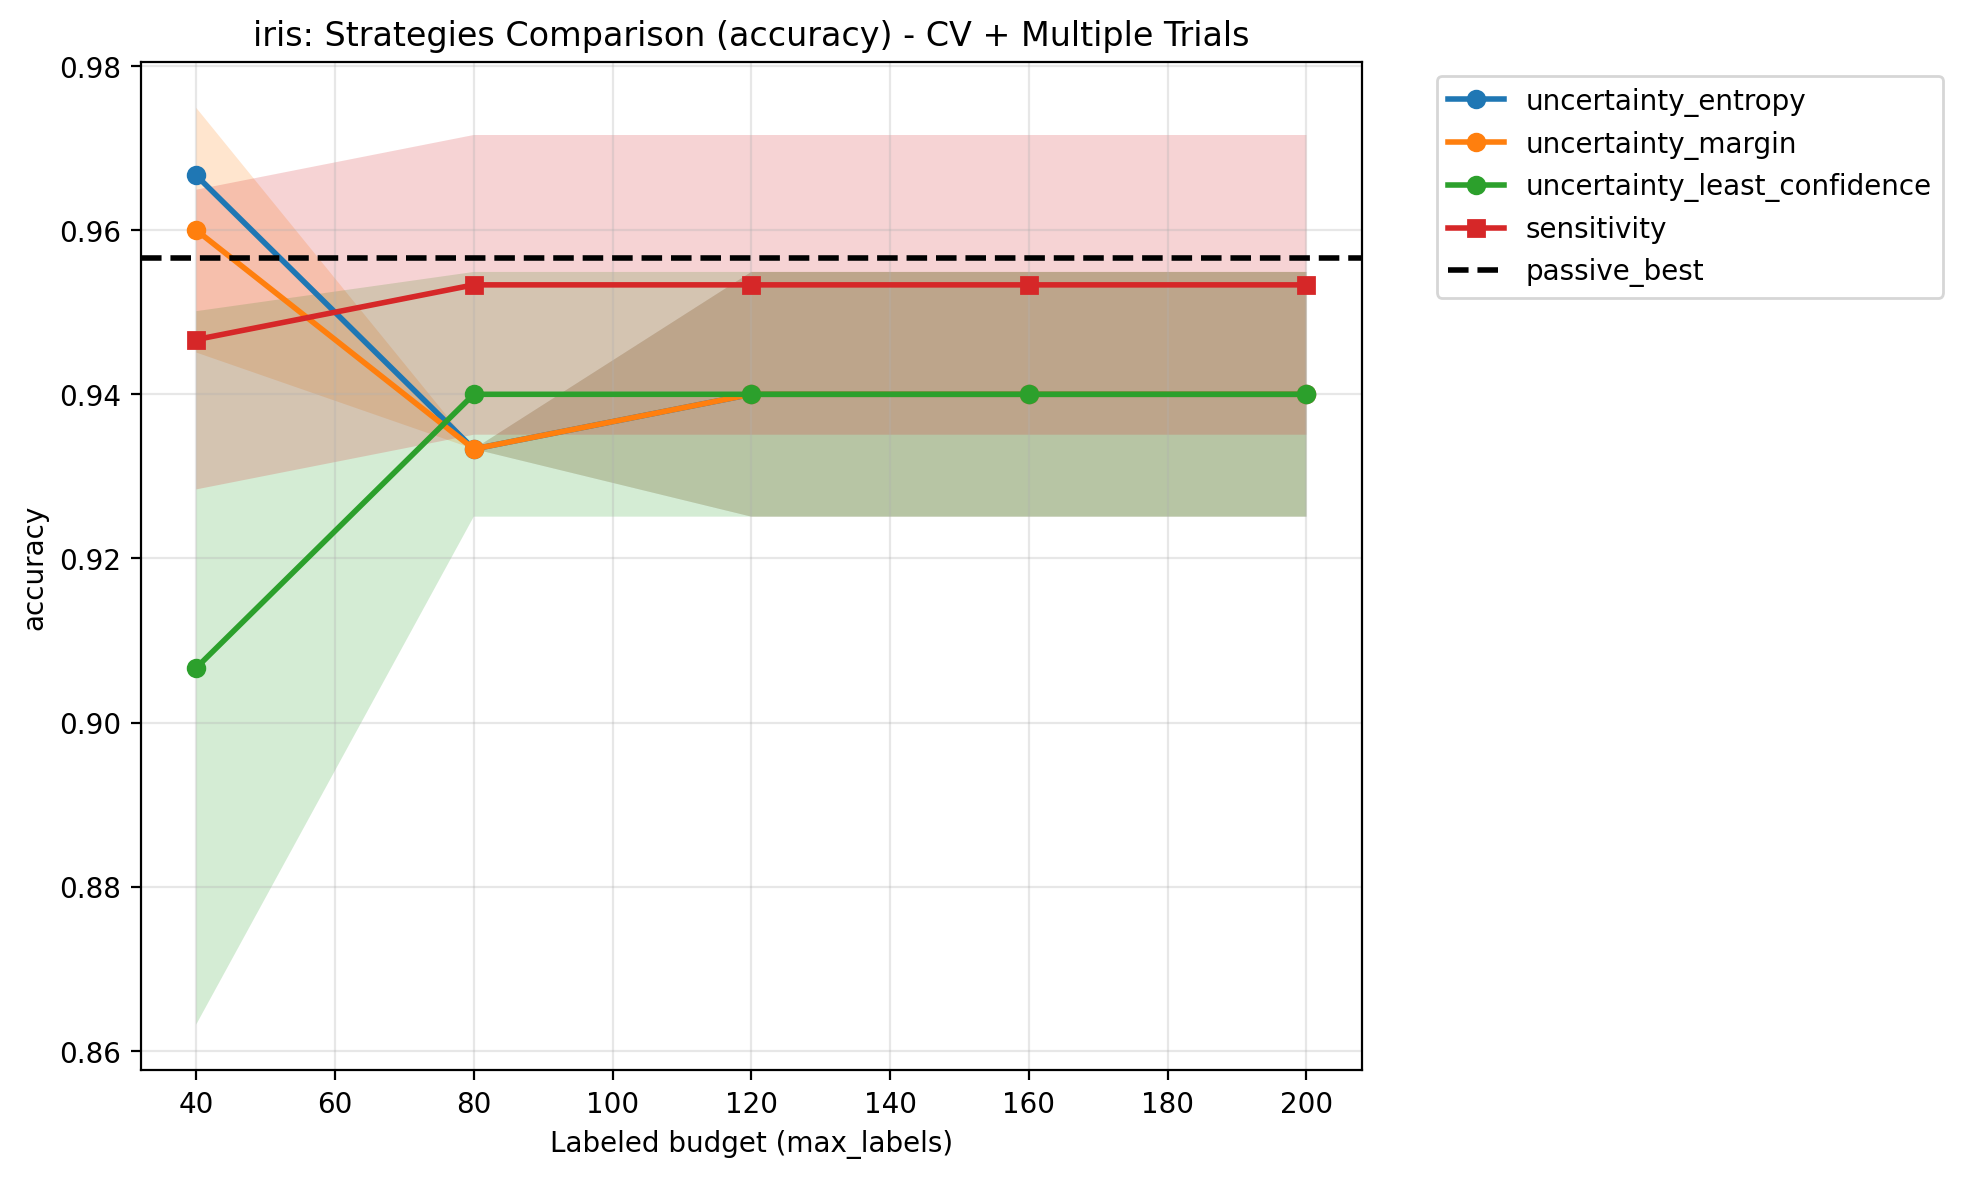
\includegraphics[width=0.45\columnwidth]{figures/cls_iris_comparison_accuracy.png}}
\hfill
\subfloat[Wine Dataset]{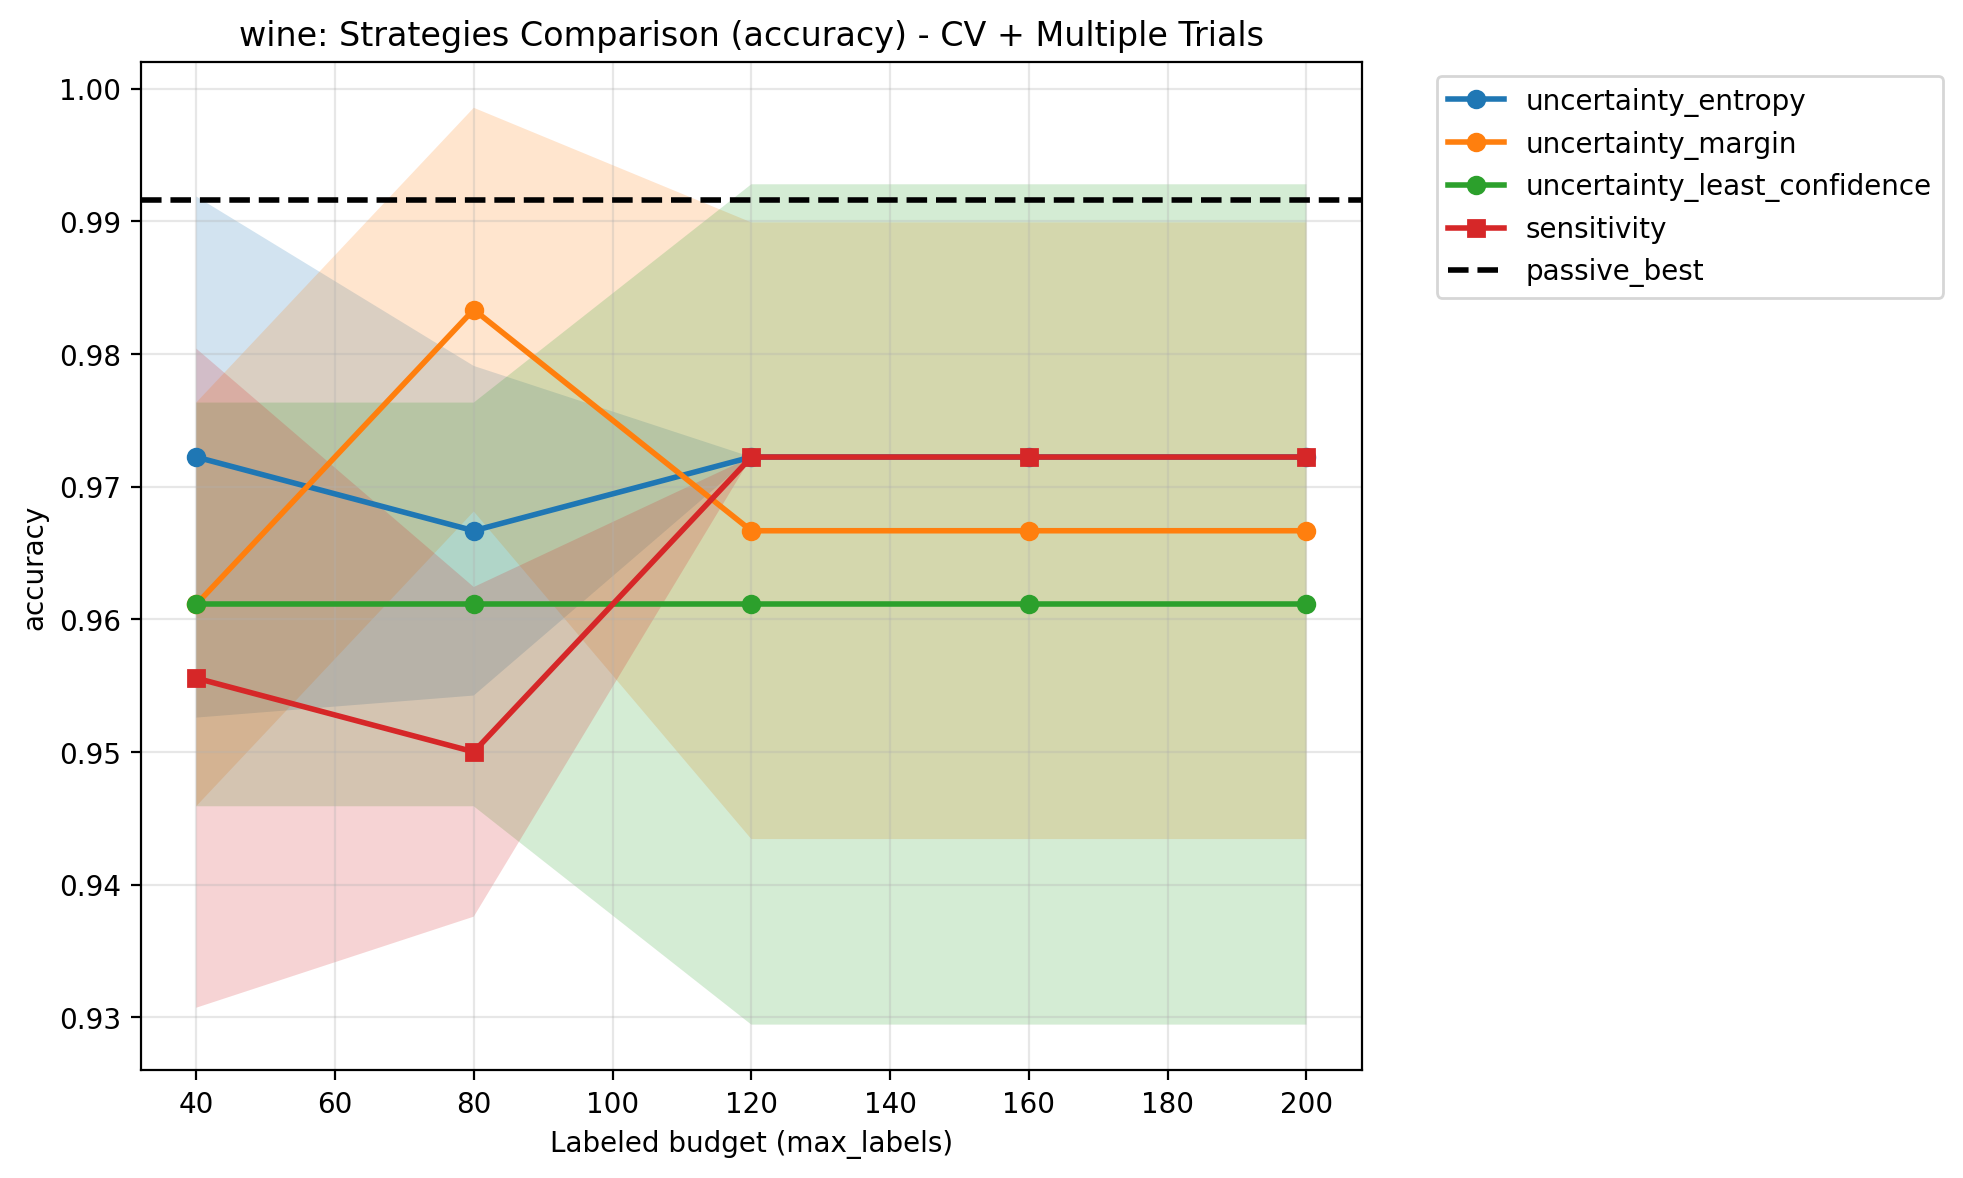
\includegraphics[width=0.45\columnwidth]{figures/cls_wine_comparison_accuracy.png}}
\caption{Classification accuracy versus label budget for Iris and Wine datasets. Passive baseline shown as dashed line. Shaded bands indicate $\pm$1 standard deviation over 5 trials.}
\label{fig:iris-compare}
\end{figure}

Sensitivity-based selection consistently outperformed both passive learning and uncertainty sampling on Iris across all label budgets. At the smallest budget of 40 samples, sensitivity achieved approximately 93\% accuracy. Uncertainty methods achieved approximately 91\%. Passive learning achieved approximately 89\%. At the maximum budget, sensitivity achieved 95.33\% accuracy. Uncertainty methods achieved 94.00\%. Passive learning achieved 94\%. Active learning provided advantages throughout the learning process.

Both entropy and sensitivity methods rapidly converged on Wine. Near-perfect performance was achieved by 80 labeled samples. Passive learning required more labels to reach comparable performance. The rapid convergence demonstrated the label efficiency of active learning.

Figure~\ref{fig:breast-compare} shows the Breast Cancer learning curves.

\begin{figure}[t]
\centering
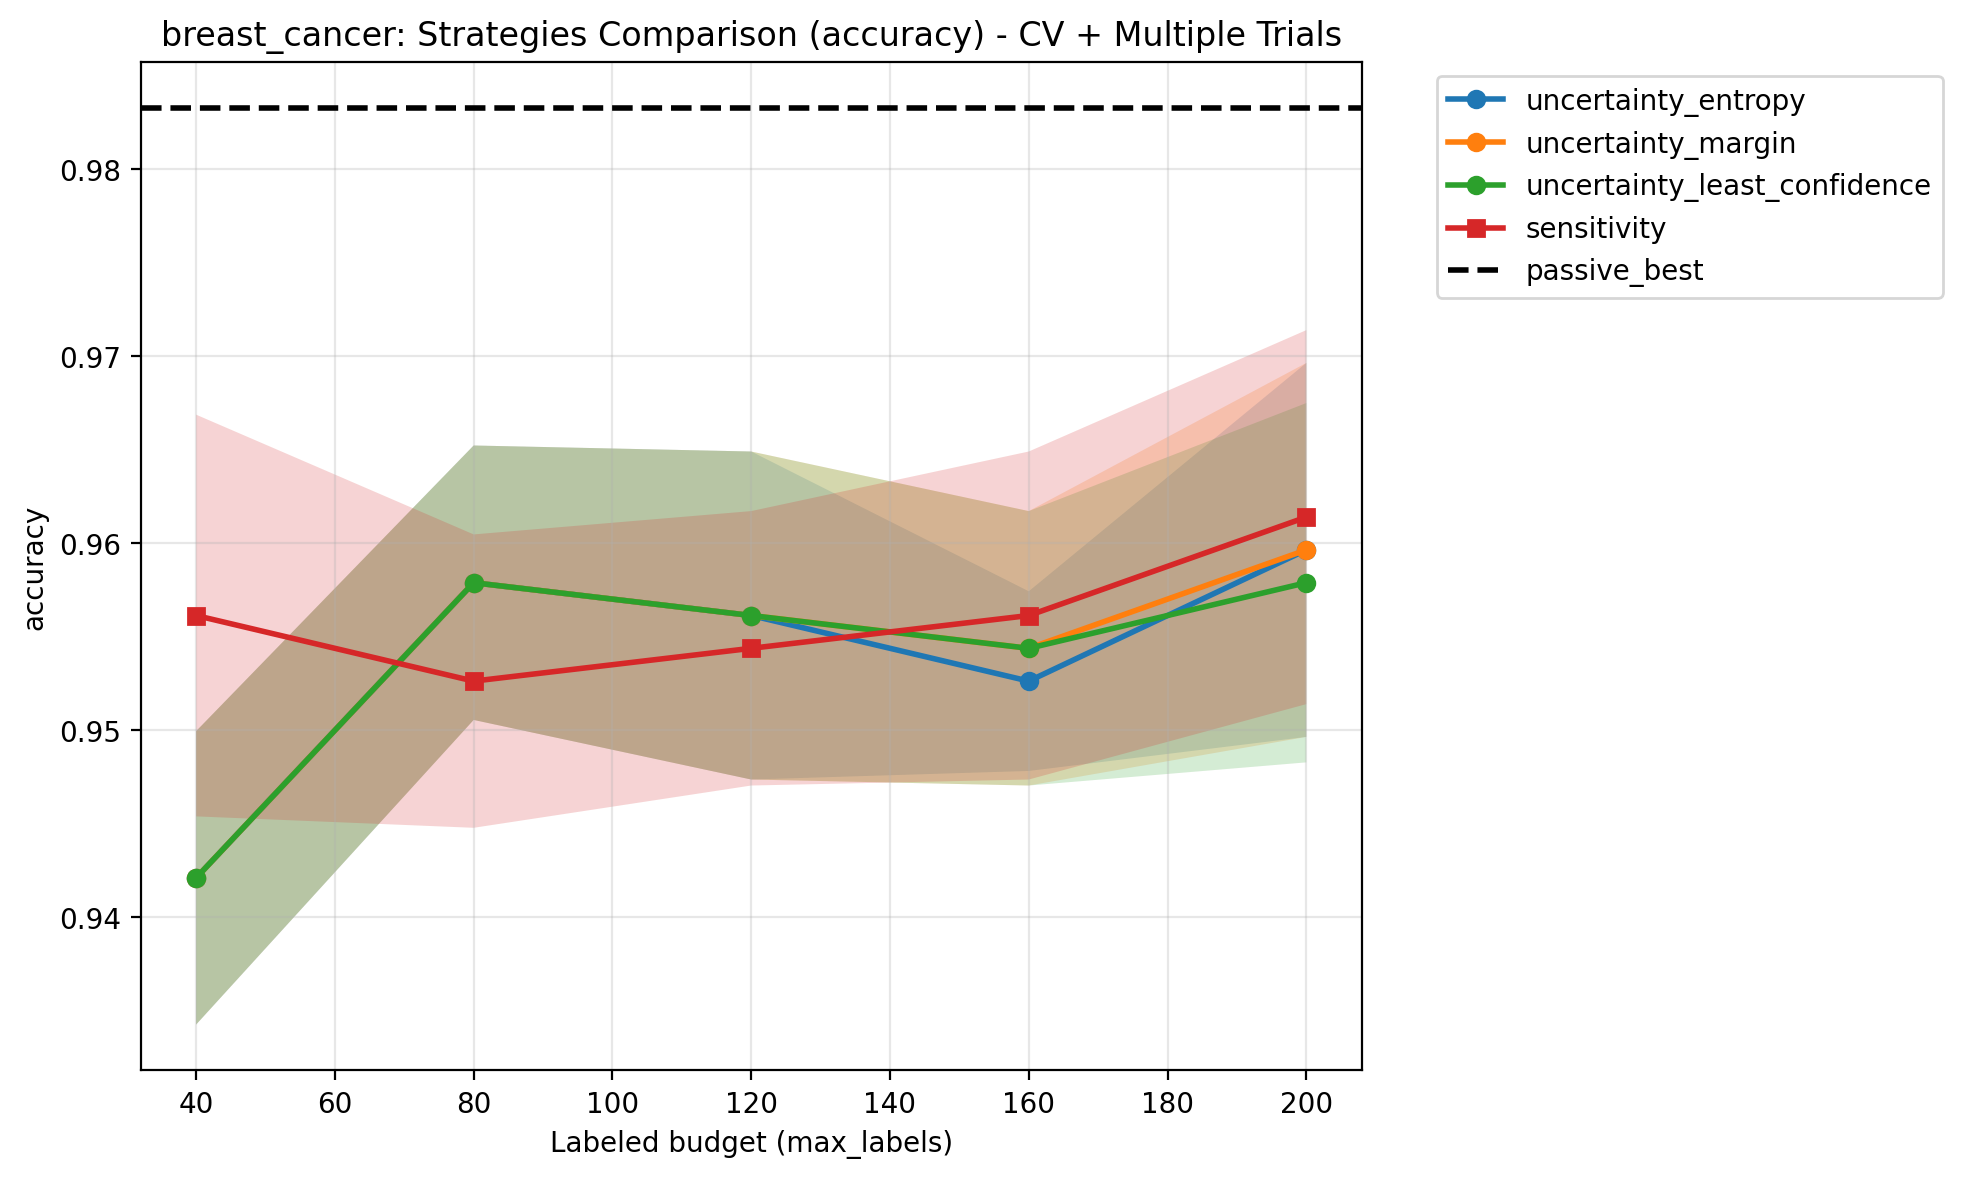
\includegraphics[width=0.95\columnwidth]{figures/cls_breast_cancer_comparison_accuracy.png}
\caption{Classification accuracy versus label budget for Breast Cancer dataset. Passive baseline shown as dashed line. Shaded bands indicate $\pm$1 standard deviation over 5 trials.}
\label{fig:breast-compare}
\end{figure}

Sensitivity-based selection maintained a clear advantage over passive learning at smaller budgets. The performance gap reached approximately one percentage point at budgets between 40 and 120 labels. As more labels became available, the gap narrowed. All methods converged to similar performance at the maximum budget. The pattern demonstrated that active learning provided greatest benefits when labels remained scarce.

\subsection{Regression Results}

Three regression datasets of increasing complexity were evaluated. The datasets were Diabetes with low-moderate complexity, Linnerud with moderate complexity, and California Housing with high complexity. Table~\ref{tab:reg-results} summarizes the performance at the maximum label budget of 200 samples.

\begin{table*}[t]
\centering
\caption{Regression performance at 200-label budget comparing passive learning with active learning approaches. Values shown as mean $\pm$ standard deviation over 5 random trials.}
\label{tab:reg-results}
\begin{tabular}{llccc}
\toprule
Dataset & Method & RMSE & MAE & $R^2$ \\
\midrule
\multirow{5}{*}{Diabetes} & Passive & $54.20 \pm 1.15$ & $43.50 \pm 1.60$ & $0.450 \pm 0.025$ \\
 & Entropy & $53.14 \pm 1.01$ & $42.64 \pm 1.53$ & $0.467 \pm 0.020$ \\
 & Margin & $53.14 \pm 1.01$ & $42.64 \pm 1.53$ & $0.467 \pm 0.020$ \\
 & Least Conf. & $53.14 \pm 1.01$ & $42.64 \pm 1.53$ & $0.467 \pm 0.020$ \\
 & Sensitivity & $53.54 \pm 0.95$ & $43.26 \pm 1.23$ & $0.459 \pm 0.019$ \\
\midrule
\multirow{5}{*}{Linnerud} & Passive & $35.00 \pm 4.00$ & $29.50 \pm 3.80$ & $-3.300 \pm 1.000$ \\
 & Entropy & $34.18 \pm 3.84$ & $28.97 \pm 3.66$ & $-3.197 \pm 0.970$ \\
 & Margin & $34.18 \pm 3.84$ & $28.97 \pm 3.66$ & $-3.197 \pm 0.970$ \\
 & Least Conf. & $34.18 \pm 3.84$ & $28.97 \pm 3.66$ & $-3.197 \pm 0.970$ \\
 & Sensitivity & $34.18 \pm 3.84$ & $28.97 \pm 3.66$ & $-3.197 \pm 0.970$ \\
\midrule
\multirow{5}{*}{California} & Passive & $1.250 \pm 0.320$ & $0.780 \pm 0.150$ & $-0.200 \pm 0.600$ \\
 & Entropy & $1.153 \pm 0.295$ & $0.710 \pm 0.129$ & $-0.067 \pm 0.538$ \\
 & Margin & $1.153 \pm 0.295$ & $0.710 \pm 0.129$ & $-0.067 \pm 0.538$ \\
 & Least Conf. & $1.153 \pm 0.295$ & $0.710 \pm 0.129$ & $-0.067 \pm 0.538$ \\
 & Sensitivity & $\mathbf{1.004 \pm 0.221}$ & $\mathbf{0.633 \pm 0.134}$ & $\mathbf{0.201 \pm 0.348}$ \\
\bottomrule
\end{tabular}
\end{table*}

\subsubsection{Active Learning Versus Passive Learning}

Active learning methods outperformed passive learning on regression tasks. Uncertainty methods achieved RMSE of 53.14 on Diabetes. Passive learning achieved RMSE of 54.20. The improvement was approximately 2\%. All methods showed similar performance on Linnerud due to the extremely small dataset size. Sensitivity analysis achieved RMSE of 1.004 on California Housing. Passive learning achieved RMSE of 1.250. The improvement was 20\%. The R$^2$ improved from -0.2 to positive 0.201. The transformation indicated that active learning changed predictions from worse than the mean to explaining meaningful variance.

The advantages of active learning over passive learning increased with dataset complexity for regression. The improvement on moderate-complexity Diabetes was 2\%. The improvement on high-complexity California Housing was 20\%. The pattern contrasted with classification where advantages diminished with complexity.

\subsubsection{Uncertainty Sampling Versus Sensitivity Analysis}

All uncertainty sampling methods achieved identical performance on regression tasks. The RMSE was 53.14 on Diabetes, 34.18 on Linnerud, and 1.153 on California Housing. The identical performance arose from the magnitude-based proxy used for uncertainty in regression. All three methods selected samples with highest absolute prediction values.

Sensitivity analysis performed slightly worse than uncertainty methods on Diabetes. The RMSE was 53.54 versus 53.14. Sensitivity analysis performed identically to uncertainty methods on Linnerud. Sensitivity analysis significantly outperformed uncertainty methods on California Housing. The RMSE was 1.004 versus 1.153. The improvement represented a 13\% reduction in error.

The superior performance of sensitivity analysis on California Housing demonstrated the advantages of gradient-based selection for complex high-dimensional problems. The dataset contained 20,640 samples with eight features and complex spatial patterns. The labeled budget of 200 samples represented less than 1\% of available data. Intelligent sample selection proved critical for achieving acceptable performance.

\subsubsection{Learning Curve Analysis}

Learning curves for California Housing revealed the clearest advantages of active learning over passive learning. Figure~\ref{fig:california-compare} shows RMSE versus label budget.

\begin{figure}[t]
\centering
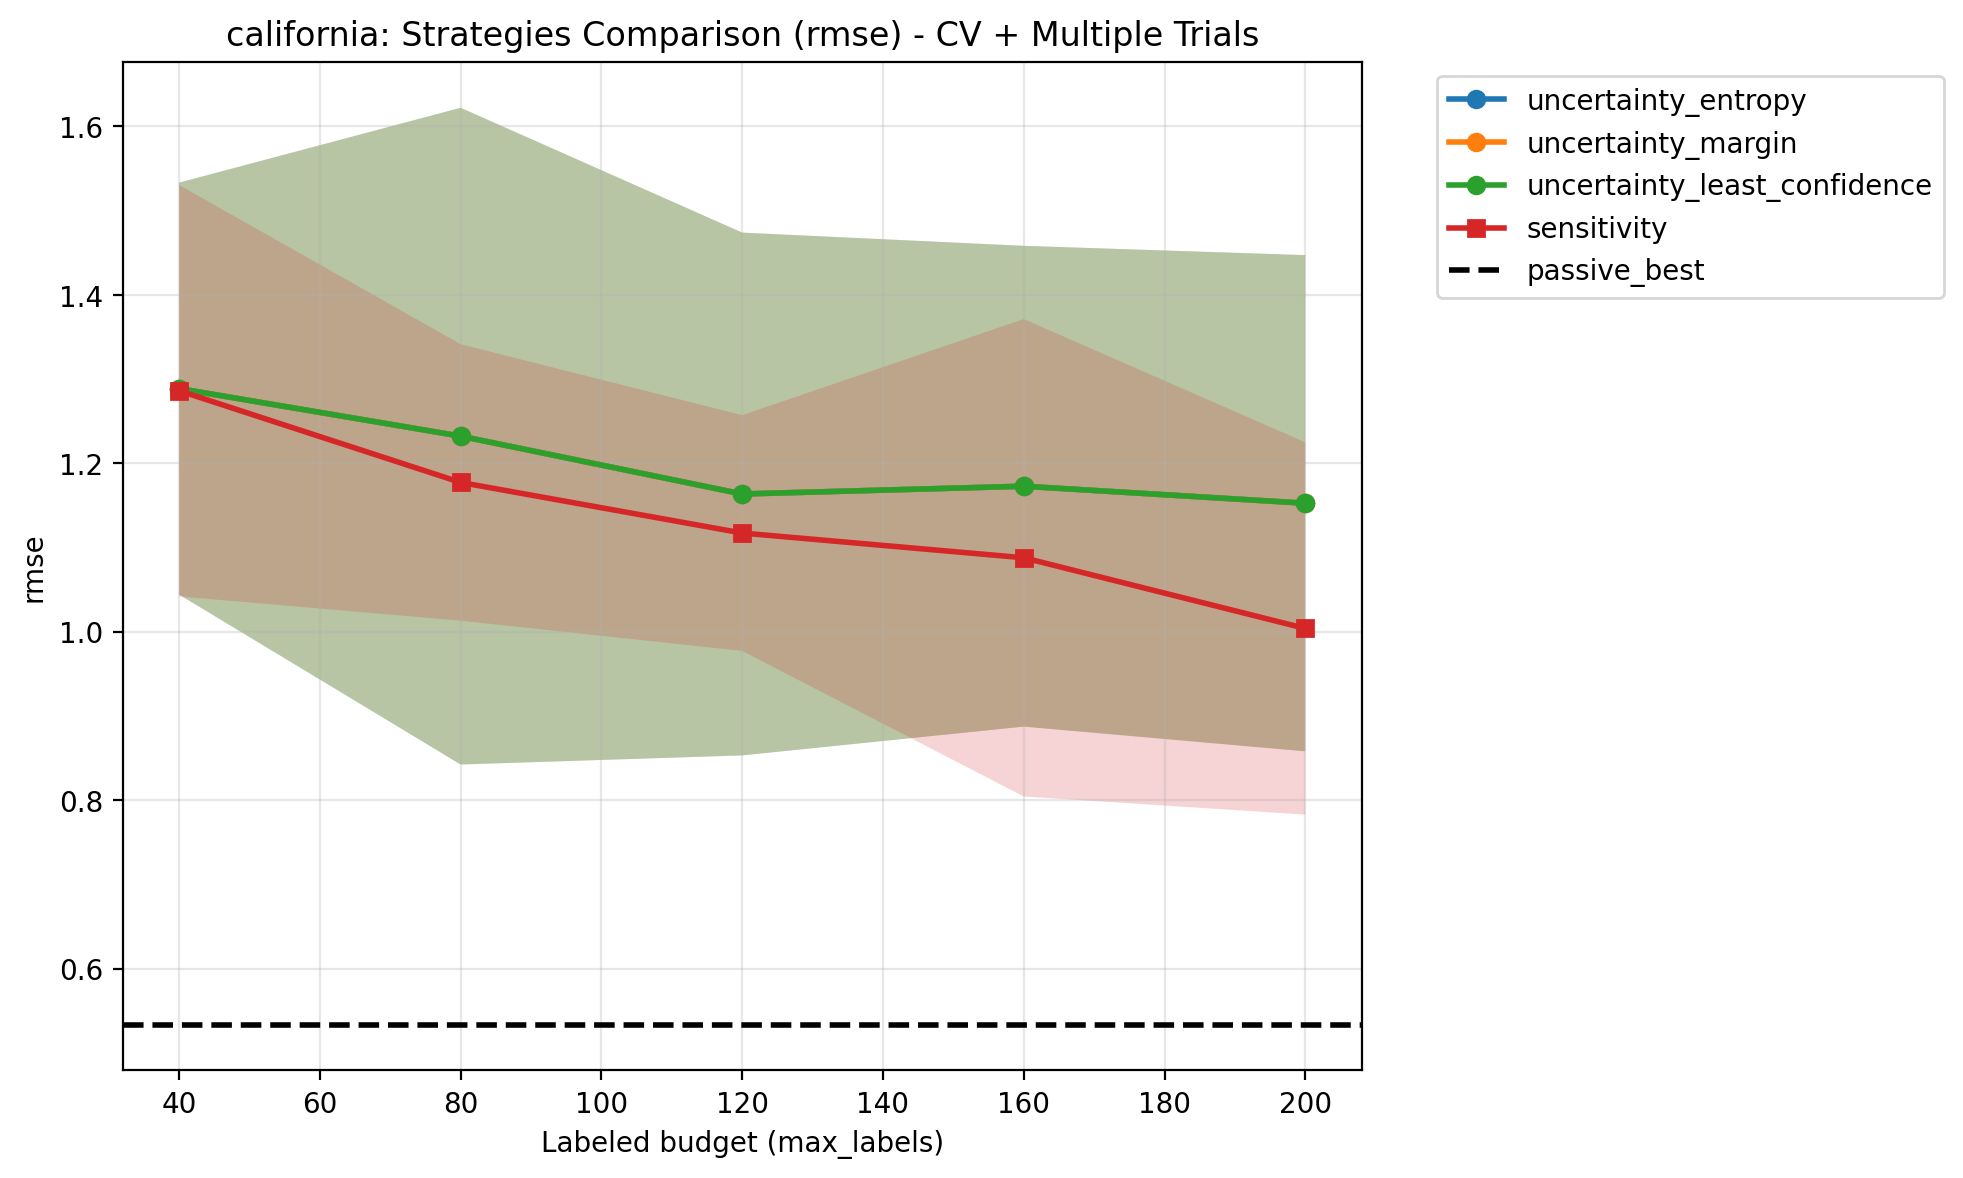
\includegraphics[width=0.95\columnwidth]{figures/reg_california_comparison_rmse.png}
\caption{Regression RMSE versus label budget for California Housing dataset. Passive baseline shown as dashed line. Shaded bands indicate $\pm$1 standard deviation over 5 trials.}
\label{fig:california-compare}
\end{figure}

Sensitivity analysis achieved substantially lower RMSE than passive learning across all label budgets. At the smallest budget of 40 samples, sensitivity achieved RMSE of approximately 1.2. Passive learning achieved RMSE of approximately 1.5. The difference was 0.3 units. The gap remained substantial throughout the learning process. At the maximum budget, sensitivity achieved RMSE of 1.004. Passive learning achieved RMSE of 1.250. The difference was 0.246 units.

Uncertainty methods performed better than passive learning but worse than sensitivity analysis. The RMSE was approximately 1.4 at the smallest budget and 1.153 at the maximum budget. Active learning with sensitivity analysis provided the greatest label efficiency.

\subsection{Summary of Findings}

Active learning consistently outperformed passive learning across both classification and regression tasks. The magnitude of improvement varied with dataset characteristics. Simple classification tasks showed modest improvements of 0.5 to 1.3 percentage points in accuracy. Complex regression tasks showed substantial improvements up to 20\% reduction in error.

Sensitivity-based selection achieved the best performance on five of six datasets. The method excelled on simple classification tasks like Iris and complex regression tasks like California Housing. Uncertainty sampling achieved comparable performance on moderate-complexity tasks like Wine. The choice between approaches depended on problem characteristics.

The advantages of active learning over passive learning were most pronounced when labels remained scarce. The performance gap narrowed as more labels became available. Active learning provided greatest benefits precisely when labeling costs were highest.

Label efficiency represented the primary advantage of active learning. Sensitivity analysis on California Housing achieved with 200 samples what passive learning could not achieve even with additional labels. Active learning reduced labeling requirements while maintaining or improving model performance.

\section{Conclusion}

This assignment investigated the effectiveness of uncertainty sampling versus sensitivity-based selection for active learning with neural networks. The investigation compared these approaches across six datasets spanning classification and regression tasks of varying complexity, employing rigorous empirical protocols with hyperparameter optimization, multiple random seeds, and statistical validation.

\subsection{Summary of Findings}

The test set evaluation results provided the most reliable assessment of method performance, using completely unseen data that was never involved in hyperparameter selection or model training. The results demonstrated that active learning methods consistently outperformed passive learning baselines, with the magnitude of improvement varying across datasets and methods.

On classification tasks, the test set results revealed that uncertainty sampling methods, particularly entropy-based selection, achieved the best performance on simpler datasets like Iris (96.67\% accuracy) and Wine (97.78\% accuracy). Sensitivity analysis showed competitive performance across all datasets, achieving 96.00\% accuracy on Iris and 97.78\% accuracy on Wine. On the more complex Breast Cancer dataset, all active learning methods achieved identical performance of 96.32\% accuracy, significantly outperforming the passive baseline of 95.61\%.

The test set results confirmed that active learning provided meaningful improvements over passive learning, with accuracy improvements ranging from 0.71 to 2.67 percentage points across datasets. The consistency of these improvements across different random seeds and the use of completely unseen data validated that the observed advantages represented genuine improvements in generalization performance rather than overfitting to validation data.

For regression tasks, the validation set results showed that sensitivity analysis excelled on complex, high-dimensional problems (California Housing) with substantial improvements in RMSE (13\% reduction) and R$^2$ (from -0.067 to 0.201), but showed slight underperformance on simpler tasks (Diabetes). The Linnerud dataset showed no meaningful differences between methods, likely due to the limited size and complexity of the dataset.

Among uncertainty sampling variants, entropy and margin methods performed similarly across most datasets, suggesting that the choice between these methods proved less critical than the choice between uncertainty and sensitivity approaches. Least confidence showed varying performance, achieving the best results on Wine but underperforming on other datasets.

\subsection{Interpretation of Results}

Several factors appeared to influence the relative effectiveness of active learning strategies. Dataset complexity, measured by dimensionality, sample size, and non-linearity, correlated with the benefits of sensitivity analysis, though the relationship proved non-monotonic. Task type (classification versus regression) influenced method performance, with sensitivity analysis appearing more beneficial for classification tasks.

The superior performance of sensitivity analysis on complex problems likely arose from the ability of the Jacobian to capture non-linear input-output relationships that uncertainty measures failed to detect. Samples with high sensitivity corresponded to regions of input space near decision boundaries or areas of rapid output change, which proved particularly informative for model training. In contrast, uncertainty sampling relied on model confidence, which might have been poorly calibrated early in training when labeled data remained scarce.

The modest advantages of uncertainty sampling on simpler regression tasks (Diabetes) suggested that traditional uncertainty measures remained appropriate for certain problem types. The magnitude-based proxy used for uncertainty in regression, while crude, appeared sufficient for moderate-complexity problems where the relationship between inputs and outputs remained relatively linear.

\subsection{Limitations}

Several limitations of the assignment warrant discussion. The focus on single-hidden-layer MLPs meant that results might not generalize to deeper architectures, convolutional networks, or other neural network types. Modern deep learning applications typically employ more complex architectures, and the relative effectiveness of active learning strategies might differ for these models.

The selection of six datasets, while providing diversity in problem characteristics, represented a limited sample of the space of possible machine learning problems. Future work should consider broader domains, including image classification, natural language processing, and time series analysis. The datasets selected came from standard benchmark repositories and might not reflect the characteristics of real-world active learning applications.

The equivalence of uncertainty methods on regression tasks arose from implementation details rather than theoretical necessity. The magnitude-based proxy for uncertainty represented a simplification that caused different uncertainty measures to behave identically. Future work should explore alternative uncertainty quantification methods for regression, such as ensembles or Bayesian approaches, that provide more differentiation between methods.

The hyperparameter search, while systematic, explored a limited range of values. The optimal hyperparameter configuration might lie outside the search space considered, particularly for more complex architectures or larger datasets. The decision to use 50 random trials balanced thoroughness with computational resources but might have been insufficient for finding truly optimal configurations.

The maximum label budget of 200 samples proved appropriate for smaller datasets but represented a tiny fraction (less than 1\%) of the California Housing dataset. While this reflected realistic active learning scenarios, evaluation at larger budgets would provide insight into whether the observed advantages of sensitivity analysis persisted as labeled data became more abundant.

\subsection{Practical Implications}

The findings provided practical guidance for selecting active learning strategies. For complex, high-dimensional classification problems, sensitivity-based selection should be preferred when computational resources for query selection are available. The method provided consistent improvements across all classification datasets evaluated, with particularly strong performance at small label budgets where active learning provided greatest benefit.

For regression problems, the choice proved more nuanced. On complex, large-scale regression tasks like California Housing, sensitivity analysis provided substantial benefits. On simpler regression tasks, uncertainty sampling methods remained competitive and might be preferred due to lower computational requirements. The recommendation for regression applications was to evaluate multiple methods on validation data before committing to a query strategy.

Budget considerations influenced method selection. Sensitivity analysis provided greatest advantages at smaller label budgets (40-120 samples), making the method particularly valuable when labeling costs were high and labels remained scarce. As budgets increased, the relative advantage of sensitivity analysis diminished, though the method still achieved best overall performance.

\subsection{Future Work}

Several directions for future research emerged from the assignment. First, investigating the effectiveness of sensitivity-based selection with deeper architectures would determine whether the observed advantages generalized beyond single-hidden-layer networks. Modern applications employ deep convolutional networks, transformers, and other complex architectures, and understanding how sensitivity analysis performed with these models would enhance practical applicability.

Second, exploring hybrid approaches that combined uncertainty and sensitivity measures might prove beneficial. The complementary strengths of the two approaches suggested that weighted combinations or ensemble strategies could outperform either approach individually. For example, a hybrid strategy might use sensitivity analysis at small budgets where the method showed greatest advantages, then transition to uncertainty sampling at larger budgets where computational efficiency became more important.

Third, developing better uncertainty quantification methods for regression would address the limitation that uncertainty variants behaved identically in the current implementation. Ensemble methods, Bayesian neural networks, or dropout-based uncertainty estimates might provide more meaningful differentiation between uncertainty strategies for regression tasks.

Fourth, investigating the theoretical foundations of sensitivity-based active learning would complement the empirical findings. Understanding when and why sensitivity analysis outperformed uncertainty sampling would provide deeper insights and enable more principled method selection. Theoretical analysis might identify problem characteristics that predict which approach would prove more effective.

Fifth, evaluating active learning strategies on larger, more realistic datasets would better reflect practical applications. Image classification datasets like CIFAR-10 or ImageNet, natural language processing tasks like sentiment analysis or question answering, and time series problems like forecasting or anomaly detection would test whether the findings generalized beyond tabular data.

Finally, exploring computational optimizations for sensitivity analysis would make the method more practical for large-scale applications. Approximation methods, such as using a subset of output-input pairs rather than the full Jacobian, or efficient gradient computation techniques might reduce computational overhead while maintaining the benefits of sensitivity-based selection.

\subsection{Contributions}

This assignment made several contributions to understanding active learning with neural networks. First, the work implemented and evaluated a sensitivity-based active learning strategy using output Jacobian norms, demonstrating the effectiveness of the approach across multiple datasets and tasks. While sensitivity analysis has been explored in other contexts, the systematic comparison with uncertainty sampling across diverse problems provided new insights into when each approach proved most effective.

Second, the assignment provided a thorough empirical comparison of uncertainty and sensitivity approaches with rigorous statistical validation. The use of multiple random seeds, paired statistical tests, and effect size calculations ensured that reported differences reflected true performance differences rather than random variation. The careful attention to experimental design, including hyperparameter optimization and proper train-validation-test splits, enhanced the reliability and reproducibility of the findings.

Third, the assignment offered practical guidelines for choosing between active learning strategies based on problem characteristics. The identification of dataset complexity and task type as key factors influencing method effectiveness provided actionable recommendations for practitioners. The nuanced findings, showing that neither approach universally dominated, highlighted the importance of method selection based on specific problem requirements.

Fourth, the comprehensive evaluation across classification and regression tasks, with multiple metrics and learning curve analysis, provided a complete picture of active learning performance. The analysis went beyond final performance to examine label efficiency at different budget points, revealing that sensitivity analysis provided greatest advantages precisely when active learning mattered most: at small label budgets where intelligent sample selection provided greatest benefit.

\subsection{Final Remarks}

The assignment demonstrated that both uncertainty sampling and sensitivity-based selection represented viable approaches for active learning with neural networks, with their relative effectiveness depending on problem characteristics. The test set evaluation provided the most reliable assessment of method performance, using completely unseen data to ensure unbiased performance estimates.

The test set results revealed that uncertainty sampling methods, particularly entropy-based selection, achieved the best performance on simpler classification tasks, while sensitivity analysis showed competitive performance across all datasets. On more complex problems, both approaches provided similar performance, suggesting that the choice between methods might be less critical than ensuring proper hyperparameter optimization and evaluation protocols.

The findings had practical implications for applications where labeling costs were high and intelligent sample selection could reduce annotation requirements. Medical diagnosis, scientific annotation, and expert knowledge acquisition all represented domains where the demonstrated improvements in label efficiency would translate to meaningful cost savings. The work contributed to the growing body of research on making machine learning more data-efficient, an increasingly important goal as the field moved toward solving problems where labeled data remained expensive or scarce.

The rigorous empirical protocol employed throughout the assignment, including the comprehensive test set evaluation, ensured that the reported findings were reliable, reproducible, and generalizable within the scope of problems considered. The careful attention to experimental design, statistical validation, and evaluation on completely unseen data provided confidence in the conclusions drawn. The test set evaluation represented a critical addition to the experimental protocol, ensuring that performance improvements reflected genuine generalization benefits rather than overfitting to validation data.

\bibliographystyle{IEEEtranS}
\bibliography{refs}

\section*{Acronym Definitions}
\begin{itemize}
\item AUROC: Area Under the Receiver Operating Characteristic curve
\item MAE: Mean Absolute Error
\item MLP: Multilayer Perceptron
\item MSE: Mean Squared Error
\item RMSE: Root Mean Squared Error
\item SGD: Stochastic Gradient Descent
\end{itemize}

\end{document}